\chapter{Analýza povrchů pružným rozptylem nabitých částic}
\section{Metoda RBS}
Analytická metoda RBS (z anglického Rutherford Back Scattering) je založena na měření energetických spekter nabitých částic , pružně rzptýlených na atomech obsažených ve zkoumaném materíálu. 
Při analýze metodou RBS se zkoumaný materiál bombarduje monoenergetickými částicemi urychlenými na energii $E_0$ (typicky od stovek keV do desítek MeV). 

\begin{figure}[bthp]
  \centering
  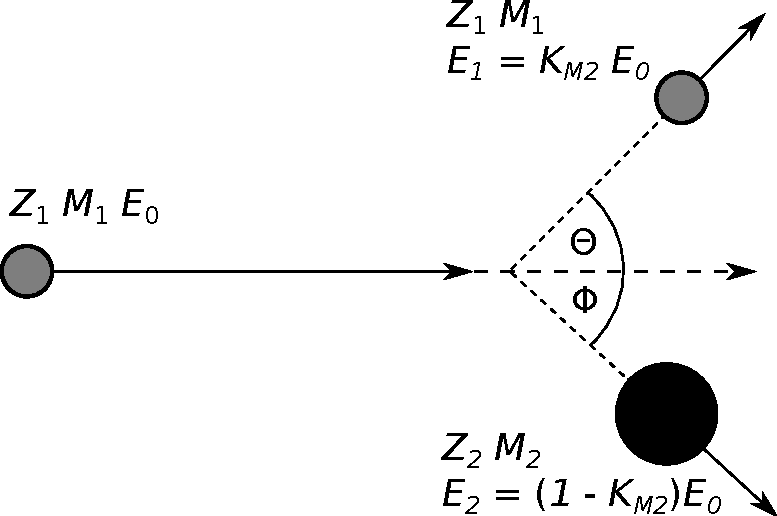
\includegraphics[width=80mm]{grafika/rutherford.pdf}
  \caption{Geometrie pružného rozptylu částice s atomovým číslem $Z_1$, hmotností $M_1$ a energií $E_0$ na atomovém jádru ($Z_2$, $M_2$), převzato z \cite{Kral2002}}
  \label{rutherford}
\end{figure}

Některé z dopadajících částic se rozptýlí na atomech obsažených v látce a jsou analyzovány spektrometrem, který určí jejich energii. Při pružném rozptylu předává částice část své kinetické energie atomu, ale celková kinetická energie soustavy částice--atom se zachovává. Energie předaná atomu závisí pouze na hotnostech částice $M_1$, atomu $M_2$ a na úhlu rozptylu $\Theta$. Z jednoduché kinematické úvahy vyplývají pro energie rozptýlené částice $E_1$ a atomu po srážce $E_2$ vztahy
%
\begin{equation}
E_1 = K_{M_2} E_0 \text{,}
\end{equation}
\begin{equation}
E_2 = (1 - K_{M_2}) E_0 \text{,}
\end{equation}  
%
kde $K_{M_2}$ je tzv. kinematický faktor a je dán vztahem
\begin{equation}
K_{M_2} = \left[ \frac{\sqrt{M_2^2 - M_1^2\sin^2\Theta} + M_1 \cos\Theta}{M_1 + M_2} \right]^2 \text{,}
\end{equation}
schéma srážky je na obrázku \ref{rutherford}.

Další, z hlediska analytického využití metody RBS významnou veličinou je účinný průřez pružného rozptylu, který spojuje počet rozptýlených částic s počtem atomů v látce. Ve standardním uspořádání metody RBS může být pružný rozptyl popsán s dostatečnou přesností jako rozptyl částice v centrálním elektrostatickém poli nestíněného atomového jádra. V takovém případě je diferenciální účinný průřez rozptylu pod laboratorním úhlem $\Theta$ dán vztahem
\begin{equation}
\frac{\mathrm{d}\sigma_\mathrm{R}}{\mathrm{d}\Omega} = 
\left( \frac{Z_1 Z_2 e^2}{2 E_0} \right)^2
 \frac{ \left[ \sqrt{M_2^2 - M_1^2\sin^2\Theta} + M_2 \cos\Theta \right]^2 }{M_2 \sin^4 \Theta \sqrt{M_2^2 - M_1^2\sin^2\Theta}}  \text{,}
\end{equation}
kde $e$ je elementární náboj. Tento vztah pro účinný průřez nicméně platí pouze v případě, kdy částice pronikne až do blízkosti jádra rozptylujícího atomu a při rozptylu lze zanedbat stínící efekt elektronového obalu. Při analýzách pomocí těžších částic a při nižších energiích může elektronové stínění hrát významnější roli. Pro vysoké energie částic a pro částice s nižším atomovým číslem naopak musíme vzít od úvahy interakce částice s atomovým jádrem prostřednictvím jaderných sil.

V nejjednodušším uspořádání, při kterém zanedbáváme energetickou závislost účinného průřezu tzv. povrchové aproximaci, můžeme pro počet detekovaných rozptýlených částic $Y$ psát
\begin{equation}
Y = \rho_S q \omega \sigma \text{,}
\end{equation}
kde $q$ je to částic, $\omega$ značí prostorový úhel detektoru a$ \rho_S$ udává plošnou hustotu atomů prvku ve vrstvě. Střední účinný průřez $\sigma$ se získá integrací diferenciálního účinného průřezu přes prostorový úhel detektoru $\omega$
\begin{equation}
\sigma = \frac{1}{\omega} \int_\omega \frac{\mathrm{d}\sigma_\mathrm{R}}{\mathrm{d}\Omega} \mathrm{d}\Omega \text{.}
\end{equation}




\section{Detekce vyražených atomů - metoda ERDA}
\begin{figure}[bthp]
  \centering
  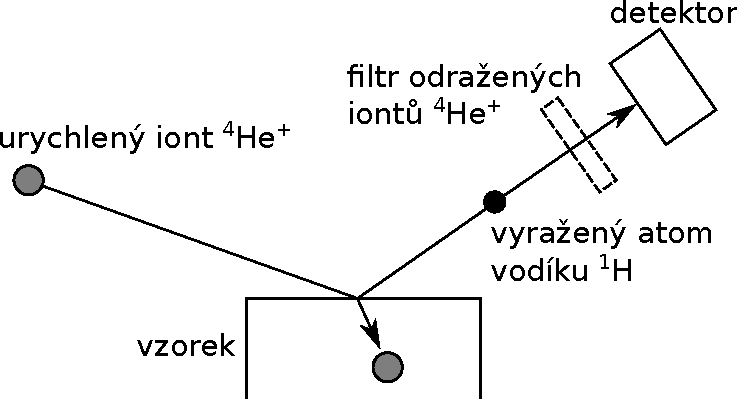
\includegraphics[width=90mm]{grafika/ERDA.pdf}
  \caption{Schéma metody ERDA pro měření vodíku, převzato z \cite{Kral2002}}
  \label{ERDA}
\end{figure}

Detekce lehkých prvků metodou RBS je obtížná vzhledem k nízkým účinným průřezům elastického rozptylu a často i proto, že příslušný analytický signál leží na vysokém pozadí vzniklém rozptylem částice na těžších prvcích. 
V případě, kdy částice mají větší hmotnost než atomy látky, k jejich rozptylu do velkých úhlů nedochází vůbec a analýza standardním postupem není možná. V takovém případě lze s výhodou použít metodu ERDA, která je založena na registraci a energetické analýze atomů vyražených dopadajícími částicemi z analyzované látky. 
Metoda ERDA je tedy postupem inverzním k běžné metodě RBS. Princip detekce atomů vodíku v nejjednodušší variantě metoda ERDA je znázorněn na obrázku \ref{ERDA}. Na vzorek dopadají monoenergetické částice $\alpha$ pod malým úhlem, zpravidla menším než 15$^\circ$ vzhledem k povrchu. 
Při jejich elastickém rozptylu dochází k vyražení lehčích atomů vodíku ze vzorku. Tyto vyražené atomy pak mohou být registrovány a energeticky analyzovány běžným polovodičovým detektorem. 
Atomy vyražené z vrstev pod povrchem vzorky jsou registrovány s energií sníženou o energetické ztráty dopadajících části a atomů vyražených z materiálu vzorku. Z tvaru energetického spektra lze pak zjistit hloubkový koncentrační profil vodíku \cite{Kral2002}. 

\cleardoublepage
